\subsection{Working Set Study}
Caches help insulate processors against long and variable latencies to DRAM.
Unfortunately, large LLCs are difficult to implement directly on FPGAs due to
area limitations. \PNAME enables the architect to explore cache sizes that
would otherwise be impossible to host on a single FPGA. We explore this by
sweeping LLC-cache sizes from \wunits{64}{KiB} to \wunits{1}{MiB} in size. In
Figure~\ref{fig:llc-speedup} we show the speed up provided by different cache
sizes and contrast them against a cache-less and single-cycle memory-system.

\begin{figure}[t]
    \centering
    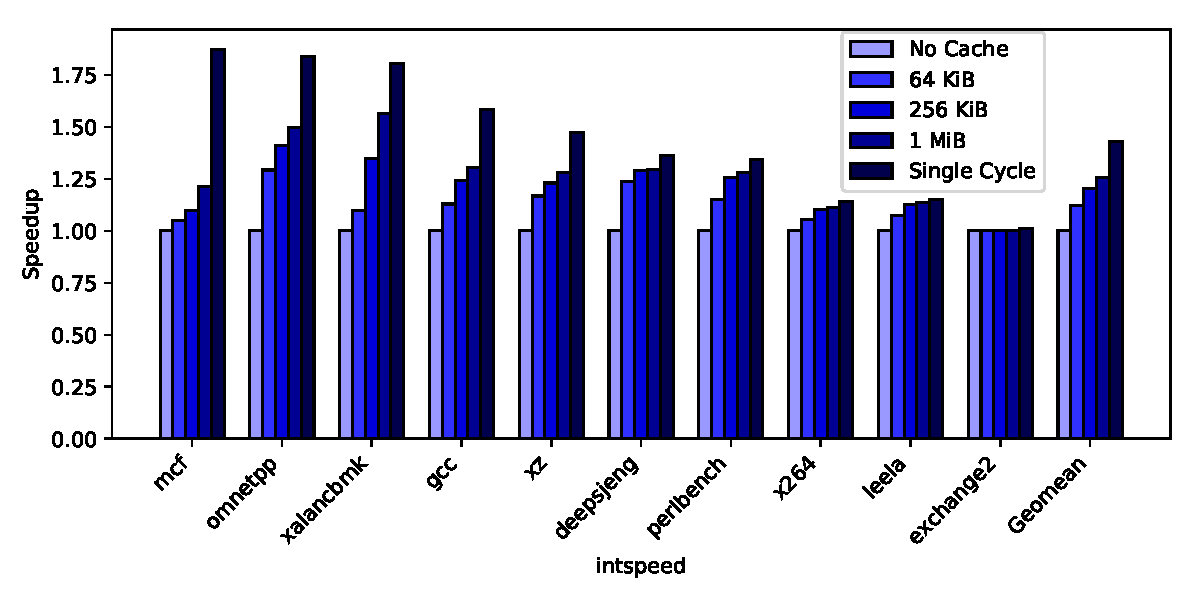
\includegraphics[width=\columnwidth]{figures/cache_size_bar_plot.pdf}
    \caption{Speedup in SPEC2017 intspeed~(reference inputs) due to different LLC sizes. All caches are 8-way set associative.}
    \label{fig:llc-speedup}
\vspace{-0.15in}
\end{figure}

\subsection{Effects of DRAM Limitations}

In this experiment, we quantify the extent to which specific timing details
affect execution time. We start with the validated model, \emph{Full}, and
gradually strip out features: \emph{No Refresh} disables refresh, \emph{No ACT
Limits} sets $t_{FAW}$ and $t_{RRD}$ to zero, and finally, \emph{Ideal} removes
all other timing considerations\footnote{$t_{RTP}$, $t_{WTR}$,
$t_{RTRS}$, $t_{RTP}$=0; $t_{RAS} = t_{RCD} + t_{CS}$ $t_{RC} =
t_{CS} + t_{RCD} + t_{RP}$.}.

\begin{figure*}
    \centering
    \begin{subfigure}[t]{0.49\textwidth}
        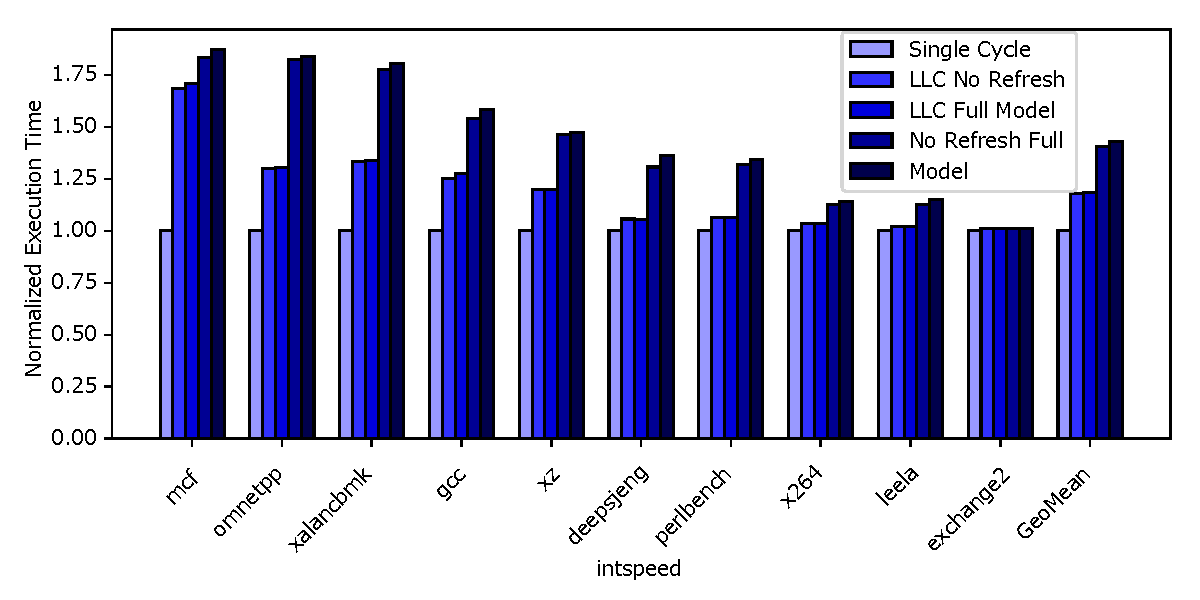
\includegraphics[width=\columnwidth]{figures/dram_fidelity_speed_slowdown.pdf}
    \end{subfigure}
    \begin{subfigure}[t]{0.49\textwidth}
        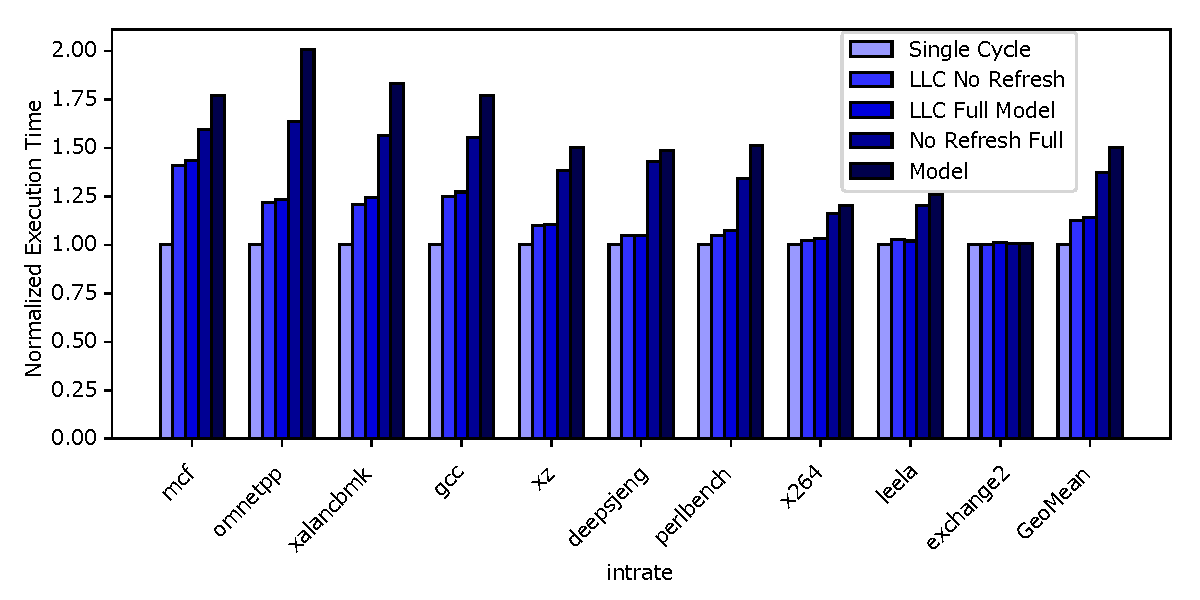
\includegraphics[width=\columnwidth]{figures/dram_fidelity_rate_slowdown.pdf}
    \end{subfigure}
    \caption{Target-execution time of SPEC2017 intspeed and intrate~(4 copies)
    with reference inputs for DRAM models with and without refresh enabled.
    Runtime is normalized to that of a single-cycle memory system. LLCs, if
    present, are \wunits{256}{KiB} and \wunits{1}{MiB} large for intspeed and
    intrate respectively and are 8-way set associative.}
    \label{fig:model-fidelity-sweep}
\end{figure*}

The slowdowns of these models relative to a single-cycle memory system are
shown in Figure~\ref{fig:model-fidelity-sweep}. Without an LLC, the largest
source of slowdown is refresh, which contributes a $1.01\times$ and
$1.11\times$ slowdown for intspeed and intrate, respectively.  Eliminating $t_{RRD}$ and $t_{FAW}$ had almost no effect; we
suspect reducing rank count and increasing device density would further induce these
effects.  Remaining DRAM non-idealities contribute $1.02\times$ slowdown.  Once
a cache is included, these effects are effectively mitigated: refresh
contributes a only $1.01\times$ slowdown in intrate.

\subsection{Simulation Performance}

%\begin{table*}[t]
%\tabcolsep=0.10cm
%\centering
%    \begin{tabular}{l
%        S[table-format=2.0]@{\hskip 0.1in}S[table-format=3.0]@{\hskip 0.11in}
%        S[table-format=2.0]@{\hskip 0.1in}S[table-format=3.0]@{\hskip 0.11in}
%        S[table-format=2.0]@{\hskip 0.1in}S[table-format=3.0]@{\hskip 0.11in}
%        S[table-format=2.0]@{\hskip 0.1in}S[table-format=3.0]@{\hskip 0.11in}
%        S[table-format=2.0]@{\hskip 0.1in}S[table-format=3.0]@{\hskip 0.11in}
%        S[table-format=2.0]@{\hskip 0.1in}S[table-format=3.0]@{\hskip 0.11in}
%        S[table-format=2.0]@{\hskip 0.1in}S[table-format=3.0]@{\hskip 0.11in}
%        S[table-format=2.0]@{\hskip 0.1in}S[table-format=3.0]@{\hskip 0.11in}
%        S[table-format=2.0]@{\hskip 0.1in}S[table-format=3.0]@{\hskip 0.11in}
%        S[table-format=2.0]@{\hskip 0.1in}S[table-format=3.0]@{\hskip 0.11in}
%    }
%\hline
%      Benchmark &
%         \multicolumn{2}{c}{{\hskip -0.08in}perlbench} &
%         \multicolumn{2}{c}{{\hskip -0.08in}gcc} &
%         \multicolumn{2}{c}{{\hskip -0.08in}mcf} &
%         \multicolumn{2}{c}{{\hskip -0.08in}omnetpp} &
%         \multicolumn{2}{c}{{\hskip -0.08in}xalancbmk} &
%         \multicolumn{2}{c}{{\hskip -0.08in}x264} &
%         \multicolumn{2}{c}{{\hskip -0.08in}deepsjeng} &
%         \multicolumn{2}{c}{{\hskip -0.08in}leela} &
%         \multicolumn{2}{c}{{\hskip -0.08in}exchange2} &
%         \multicolumn{2}{c}{{\hskip -0.08in}xz} \\
%        Model &
%        hr &   MHz &
%        hr &   MHz &
%        hr &   MHz &
%        hr &   MHz &
%        hr &   MHz &
%        hr &   MHz &
%        hr &   MHz &
%        hr &   MHz &
%        hr &   MHz &
%        hr &  MHz \\
%\hline
%        Single Cycle &  14.4 &   95 &  20.4 &   73 &  24.7 &   62 &    13.8 &   67 &      14.0 &   68 &  12.9 &  123 &      13.4 &   87 &   8.6 &  119 &       6.9 &  153 &  50.5 &  90 \\
%        FCFS, 256KB LLC     &      14.7 &  100 &  20.8 &  91 &  25.6 &  102 &    14.1 &  86 &      14.5 &  88 &  13.1 &  125 &      13.6 &  91 &   8.6 &  121 &       6.9 &  153 &  51.8 &  105 \\
%        FCFS, No LLC     &      14.7 &  126 &  20.9 &  113 &  25.7 &  112 &    14.3 &  119 &      14.7 &  118 &  13.2 &  137 &      13.6 &  117 &   8.7 &  135 &       7.0 &  152 &  52.1 & 110 \\
%%Single Cycle &      14.4 &   95.8 &  20.4 &   73.3 &  24.7 &   62.1 &    13.8 &   67.4 &      14.0 &   68.6 &  12.9 &  123.0 &      13.4 &   87.5 &   8.6 &  119.0 &       6.9 &  153.3 &  50.5 &  90.5 \\
%%        FCFS, 256KB LLC     &      14.7 &  100.4 &  20.8 &  91.4 &  25.6 &  102.7 &    14.1 &  86.1 &      14.5 &  88.4 &  13.1 &  125.2 &      13.6 &  91.5 &   8.6 &  121.2 &       6.9 &  153.0 &  51.8 &  105.8 \\
%%        FCFS, No LLC     &      14.7 &  126.4 &  20.9 &  113.1 &  25.7 &  112.2 &    14.3 &  119.6 &      14.7 &  118.1 &  13.2 &  137.7 &      13.6 &  117.6 &   8.7 &  135.3 &       7.0 &  152.2 &  52.1 & 110.6 \\
%\hline
%\end{tabular}
%    \caption{Simulation times and rates for SPEC2017 intspeed running on a
%    single-core Rocket Chip target.}
%    \label{tbl:intspeed-simtimes}
%\vspace{-0.1in}
%\end{table*}
%\begin{table*}[t]
%\tabcolsep=0.10cm
%\centering
%    \begin{tabular}{l
%        S[table-format=2.0]@{\hskip 0.1in}S[table-format=3.0]@{\hskip 0.11in}
%        S[table-format=2.0]@{\hskip 0.1in}S[table-format=3.0]@{\hskip 0.11in}
%        S[table-format=2.0]@{\hskip 0.1in}S[table-format=3.0]@{\hskip 0.11in}
%        S[table-format=2.0]@{\hskip 0.1in}S[table-format=3.0]@{\hskip 0.11in}
%        S[table-format=2.0]@{\hskip 0.1in}S[table-format=3.0]@{\hskip 0.11in}
%        S[table-format=2.0]@{\hskip 0.1in}S[table-format=3.0]@{\hskip 0.11in}
%        S[table-format=2.0]@{\hskip 0.1in}S[table-format=3.0]@{\hskip 0.11in}
%        S[table-format=2.0]@{\hskip 0.1in}S[table-format=3.0]@{\hskip 0.11in}
%        S[table-format=2.0]@{\hskip 0.1in}S[table-format=3.0]@{\hskip 0.11in}
%        S[table-format=2.0]@{\hskip 0.1in}S[table-format=3.0]@{\hskip 0.11in}
%    }
%\hline
%      Benchmark &
%         \multicolumn{2}{c}{{\hskip -0.08in}perlbench} &
%         \multicolumn{2}{c}{{\hskip -0.08in}gcc} &
%         \multicolumn{2}{c}{{\hskip -0.08in}mcf} &
%         \multicolumn{2}{c}{{\hskip -0.08in}omnetpp} &
%         \multicolumn{2}{c}{{\hskip -0.08in}xalancbmk} &
%         \multicolumn{2}{c}{{\hskip -0.08in}x264} &
%         \multicolumn{2}{c}{{\hskip -0.08in}deepsjeng} &
%         \multicolumn{2}{c}{{\hskip -0.08in}leela} &
%         \multicolumn{2}{c}{{\hskip -0.08in}exchange2} &
%         \multicolumn{2}{c}{{\hskip -0.08in}xz} \\
%        Model &
%        hr &   MHz &
%        hr &   MHz &
%        hr &   MHz &
%        hr &   MHz &
%        hr &   MHz &
%        hr &   MHz &
%        hr &   MHz &
%        hr &   MHz &
%        hr &   MHz &
%        hr &  MHz \\
%\hline
%Single Cycle &      31.6 &   50 &  28.5 &  38 &  33.3 &   36 &    37.1 &  35 &      36.6 &   37 &  20.8 &   79 &      25.8 &   44 &  14.9 &   73 &       7.0 &  151 &  22.6 &   51 \\
%FRFCFS, 1MB LLC  &      31.2 &  54 &  24.4 &  57 &  23.9 &  72 &    32.5 &  49 &      31.4 &  54 &  20.4 &  84 &      24.8 &  48 &  14.3 &  78 &       7.1 &  150 &  20.7 &  62 \\
%FRFCFS, No LLC  &      21.6 &  111 &  19.6 &  98 &  20.2 &  104 &    27.3 &  96 &      22.8 &  110 &  15.9 &  125 &      15.4 &  110 &  11.4 &  120 &       7.0 &  152 &  16.4 &  107 \\ \hline
%\end{tabular}
%    \caption{Simulation times and rates for SPEC2017 intrate benchmarks with
%    four copies running on a quad-core Rocket Chip target.}
%    \label{tbl:intrate-simtimes}
%\vspace{-0.1in}
%\end{table*}

\begin{table*}[t]
\tabcolsep=0.10cm
\centering
    \resizebox{\textwidth}{!}{%
    \begin{tabular}{l@{\hskip -0.03in}l
        S[table-format=2.0]@{\hskip 0.14in}S[table-format=3.0]@{\hskip 0.15in}
        S[table-format=2.0]@{\hskip 0.14in}S[table-format=3.0]@{\hskip 0.15in}
        S[table-format=2.0]@{\hskip 0.14in}S[table-format=3.0]@{\hskip 0.15in}
        S[table-format=2.0]@{\hskip 0.14in}S[table-format=3.0]@{\hskip 0.15in}
        S[table-format=2.0]@{\hskip 0.14in}S[table-format=3.0]@{\hskip 0.15in}
        S[table-format=2.0]@{\hskip 0.14in}S[table-format=3.0]@{\hskip 0.15in}
        S[table-format=2.0]@{\hskip 0.14in}S[table-format=3.0]@{\hskip 0.15in}
        S[table-format=2.0]@{\hskip 0.14in}S[table-format=3.0]@{\hskip 0.15in}
        S[table-format=2.0]@{\hskip 0.14in}S[table-format=3.0]@{\hskip 0.15in}
        S[table-format=2.0]@{\hskip 0.14in}S[table-format=3.0]@{\hskip 0.15in}
    }
\hline
         \multicolumn{2}{c}{{\hskip -0.08in}} &
         \multicolumn{2}{c}{{\hskip -0.08in}perlbench} &
         \multicolumn{2}{c}{{\hskip -0.08in}gcc} &
         \multicolumn{2}{c}{{\hskip -0.08in}mcf} &
         \multicolumn{2}{c}{{\hskip -0.08in}omnetpp} &
         \multicolumn{2}{c}{{\hskip -0.08in}xalancbmk} &
         \multicolumn{2}{c}{{\hskip -0.08in}x264} &
         \multicolumn{2}{c}{{\hskip -0.08in}deepsjeng} &
         \multicolumn{2}{c}{{\hskip -0.08in}leela} &
         \multicolumn{2}{c}{{\hskip -0.08in}exchange2} &
         \multicolumn{2}{c}{{\hskip -0.08in}xz} \\
        & Model Type &
        hr & $f$ &
        hr & $f$ &
        hr & $f$ &
        hr & $f$ &
        hr & $f$ &
        hr & $f$ &
        hr & $f$ &
        hr & $f$ &
        hr & $f$ &
        hr & $f$ \\
\hline  
        \parbox[t]{0.2in}{\multirow{3}{*}{\rotatebox[origin=l]{90}{Speed}}}
        &Single Cycle &  14.4 &   95 &  20.4 &   73 &  24.7 &   62 &    13.8 &   67 &      14.0 &   68 &  12.9 &  123 &      13.4 &   87 &   8.6 &  119 &       6.9 &  153 &  50.5 &  90 \\
        &FCFS-256KB     &      14.7 &  100 &  20.8 &  91 &  25.6 &  102 &    14.1 &  86 &      14.5 &  88 &  13.1 &  125 &      13.6 &  91 &   8.6 &  121 &       6.9 &  153 &  51.8 &  105 \\
        &FCFS     &      14.7 &  126 &  20.9 &  113 &  25.7 &  112 &    14.3 &  119 &      14.7 &  118 &  13.2 &  137 &      13.6 &  117 &   8.7 &  135 &       7.0 &  152 &  52.1 & 110 \\
%Single Cycle &      14.4 &   95.8 &  20.4 &   73.3 &  24.7 &   62.1 &    13.8 &   67.4 &      14.0 &   68.6 &  12.9 &  123.0 &      13.4 &   87.5 &   8.6 &  119.0 &       6.9 &  153.3 &  50.5 &  90.5 \\
%        FCFS, 256KB LLC     &      14.7 &  100.4 &  20.8 &  91.4 &  25.6 &  102.7 &    14.1 &  86.1 &      14.5 &  88.4 &  13.1 &  125.2 &      13.6 &  91.5 &   8.6 &  121.2 &       6.9 &  153.0 &  51.8 &  105.8 \\
%        FCFS, No LLC     &      14.7 &  126.4 &  20.9 &  113.1 &  25.7 &  112.2 &    14.3 &  119.6 &      14.7 &  118.1 &  13.2 &  137.7 &      13.6 &  117.6 &   8.7 &  135.3 &       7.0 &  152.2 &  52.1 & 110.6 \\
\hline
        \parbox[t]{0.1in}{\multirow{3}{*}{\rotatebox[origin=l]{90}{Rate}}}
        &Single Cycle &      31.6 &   50 &  28.5 &  38 &  33.3 &   36 &    37.1 &  35 &      36.6 &   37 &  20.8 &   79 &      25.8 &   44 &  14.9 &   73 &       7.0 &  151 &  22.6 &   51 \\
        &FRFCFS-1MB  &      31.2 &  54 &  24.4 &  57 &  23.9 &  72 &    32.5 &  49 &      31.4 &  54 &  20.4 &  84 &      24.8 &  48 &  14.3 &  78 &       7.1 &  150 &  20.7 &  62 \\
        &FRFCFS  &      21.6 &  111 &  19.6 &  98 &  20.2 &  104 &    27.3 &  96 &      22.8 &  110 &  15.9 &  125 &      15.4 &  110 &  11.4 &  120 &       7.0 &  152 &  16.4 &  107 \\ \hline
    \end{tabular}}
    \caption{Simulation times (hours) and rates ($f$, MHz) for SPEC2017 intspeed and intrate~(four copies) running on single and quad-core Rocket Chip targets. In all cases, the FPGA-host frequency is 160 MHz.} 
    \label{tbl:intrate-simtimes}
\vspace{-0.1in}
\end{table*}


Table~\ref{tbl:intspeed-simtimes} and Table~\ref{tbl:intrate-simtimes} give the
host-execution times and execution speeds for a handful of SPEC2017 runs. The
targets with DDR3 models consistently run at a simulation rate above \wunits{100}{MHz}. Theoretically,
our models can operate at unity FMR~(160 MHz) if the target memory system is
slower than the host-memory system. On our host, reads and writes take on average 47
and 37 cycles, respectively, when unloaded.  Although these latencies have
a significant effect on simulator performance when modeling a single-cycle memory
system, they have relatively little impact when modeling a realistic DRAM system
whose latency is comparable to that of the host.
Instances with LLCs fall between these extremes, since LLC hits are fast
in target time but require a DRAM access on the host side.
For our DDR3-2133
target memory system, reads take 20, 34, and 48 cycles for row hits, closed
row, and row misses, respectively; for the accesses that take longer in
target time than host time, the simulator incurs no stalls.  Ironically,
modeling a slower DDR-speed-grade, say DDR3-800, results in lower simulation
rate: since $t_{CS}$ is smaller, reads complete in fewer target \emph{cycles}
despite taking more target \emph{time}.

\begin{figure*}
    \centering
    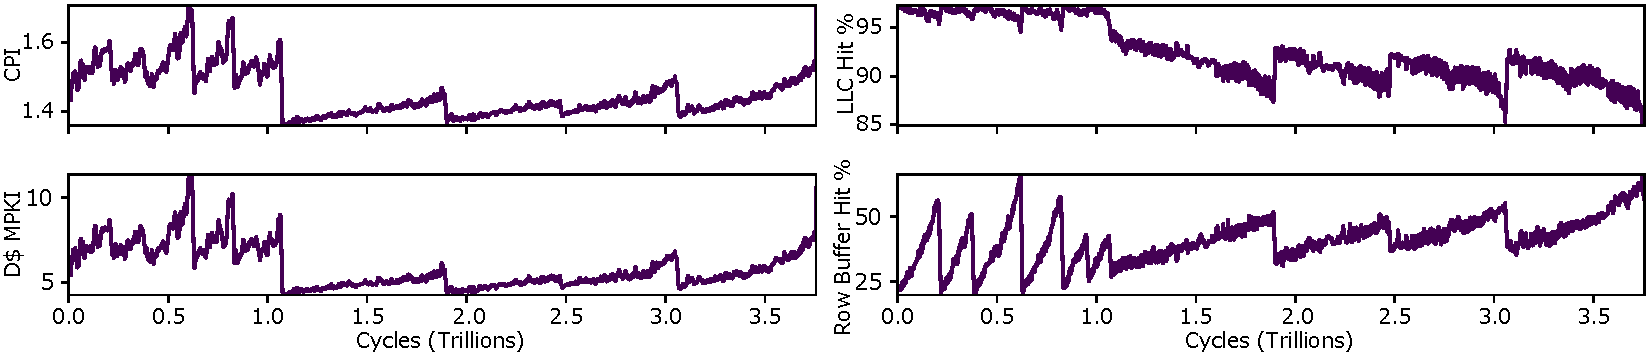
\includegraphics[width=\textwidth]{figures/leela-time-series.pdf}
    \caption{CPI, D\$ MPKI, and row buffer and LLC hit rates running
    641.leela\_s with on Rocket with \wunits{256}{KiB} of LLC and a FCFS MAS
    model. These plots use a rolling average of 10 samples spaced a billion
    cycles apart.}.
    \label{fig:leela-time-series}
\vspace{-0.1in}
\end{figure*}

\subsection{Instrumentability}
\PNAME allows the user to instrument timing models without changing target
behavior. Coupled with fast simulation speeds, this allows a \PNAME instance to
provide insight into system-wide behavior that would be difficult to collect
otherwise. We demonstrate this in Figure~\ref{fig:leela-time-series}, where we
see how row buffer and LLC hit rate are inversely correlated through each of
641.leela's games of Go.
